\section{Morphisms Between Games} \label{sec:morphisms}
There are two important reasons why our simplifying assumption that players have the same strategy labels leaves our analysis incomplete. Our first reason is that relabelling the strategies for a standard symmetric game leads to a strategically equivalent game that may no longer be considered symmetric inside our label-dependent framework. 

Ideally we want to be able to determine when two games merely differ by player and strategy labels without having to go through and check all possible rearrangements of the labels.

Our second reason is that there are weaker notions of fairness that cannot be captured within our label-dependent framework. As a motivating example consider Matching Pennies.

\begin{example} \label{MPeg}
	Matching Pennies
	\begin{center}
		\begin{game}{2}{2}
			      \> $H$    \> $T$ \\
			$H$   \> $1,-1$  \> $-1,1$ \\
			$T$   \> $-1,1$  \> $1,-1$
		\end{game} 
	\end{center}
	It is clear just by looking at the payoff matrix that Matching Pennies is fair, yet inside our label dependent framework the only invariant is the identity permutation, a problem that persists if we swap the strategy labels for either or both of the players.             
\end{example}

\subsection{Game Bijections}    
	\begin{definition}
		A \textit{game bijection} from $\Gamma_1 = (N, A, u)$ to $\Gamma_2 = (M, B, v)$ consists of a bijection $\pi:N\rightarrow M$ and for each player $i \in N$, a bijection $\tau_i:A_i\rightarrow B_{\pi(i)}$, which we denote as $\bigl(\pi; (\tau_i)_{i \in N}\bigr)$.
	\end{definition}

	More on game bijections can be found in \cite{IsoComplexity}. We denote the set of game bijections from $\Gamma_1$ to $\Gamma_2$ as $\bij(\Gamma_1, \Gamma_2)$, or simply $S_{\Gamma}$ for the bijections from a game $\Gamma$ to itself. Let $g = \bigl(\pi; (\tau_i)_{i \in N}\bigr) \in \bij(\Gamma_1, \Gamma_2)$, $i \in N$, $s_i \in A_i$ and $s \in A$, using similar notation to our label-dependent framework we denote $\pi(i)$ as $g(i)$, $\tau_i(s_i)$ as $g(s_i)$, $\bigl(\tau_{\pi^{-1}(j)}(s_{\pi^{-1}(j)})\bigr)_{j \in M} \in B$ as $g(s)$ giving $\bigl(g(s)\bigr)_{g(i)} = \tau_i(s_i) = g(s_i)$, and the map $s \mapsto u_{g(i)}\bigl(g(s)\bigr)$ as $u_{g(i)} \circ g$. 	
	
	\begin{example} \label{egisomgames}
		Consider the following $2$-player games.            
        \begin{center}
            \begin{game}{2}{2}[$\Gamma_1$]
                        \> $c$  \> $d$ \\
                $a$   \> $1,2$  \> $3,4$ \\
                $b$   \> $5,6$  \> $7,8$
            \end{game}
            \hspace*{10mm} 
            \begin{game}{2}{2}[$\Gamma_2$]
                        \> $h$ \> $i$ \\
                $e$   \> $4,3$ \> $8,7$ \\
                $f$   \> $2,1$ \> $6,5$ \\
            \end{game} 
        \end{center}
        
		Given $(a, c) \in A$ and $g = \bigl((12) ; \bigl(\begin{smallmatrix} a & b \\ h & i \end{smallmatrix}\bigr), \bigl(\begin{smallmatrix} c & d \\ f & e \end{smallmatrix}\bigr)\bigr) \in \bij(\Gamma_1, \Gamma_2)$, $g(a,c) = (f,h)$.
	\end{example}
        
	Let $\Gamma_3 = (L, C, w)$ also be a game. For $g = \bigl(\pi; (\tau_i)_{i \in N}\bigr) \in \bij(\Gamma_1, \Gamma_2)$ and $h = \bigl(\eta; (\phi_j)_{j \in M}\bigr) \in \bij(\Gamma_2, \Gamma_3)$, their \textit{composite}, denoted $h\circ g$, is $\bigl(\eta\circ\pi; (\phi_{\pi(i)}\circ\tau_i)_{i \in N}\bigr) \in \bij(\Gamma_1, \Gamma_3)$, and the \textit{inverse} of $g$, denoted $g^{-1}$, is $\bigl(\pi^{-1}; (\tau^{-1}_{\pi^{-1}(j)})_{j \in M}\bigr) \in \bij(\Gamma_2, \Gamma_1)$.   
   	
   	\begin{example}
   		Consider Example \ref{stdsymeg} except with strategy labels $A_2 =\{c, d\}$ and $A_3 = \{e, f\}$ for players $2$ and $3$ respectively. We compose and invert bijections $g = \bigl((123) ; \bigl(\begin{smallmatrix} a & b \\ d & c \end{smallmatrix}\bigr), \bigl(\begin{smallmatrix} c & d \\ e & f \end{smallmatrix}\bigr), \bigl(\begin{smallmatrix} e & f \\ b & a \end{smallmatrix}\bigr)\bigr)$, $h = \bigl((12) ; \bigl(\begin{smallmatrix} a & b \\ c & d \end{smallmatrix}\bigr), \bigl(\begin{smallmatrix} c & d \\ a & b \end{smallmatrix}\bigr), \bigl(\begin{smallmatrix} e & f \\ f & e \end{smallmatrix}\bigr)\bigr) \in S_{\Gamma}$ as follows:
   		\begin{align*}
   			%g(b,d,e) &= (a,c,f) \\
   			h \circ g &= \bigl((12) ; \bigl(\begin{smallmatrix} a & b \\ c & d \end{smallmatrix}\bigr), \bigl(\begin{smallmatrix} c & d \\ a & b \end{smallmatrix}\bigr), \bigl(\begin{smallmatrix} e & f \\ f & e \end{smallmatrix}\bigr)\bigr) \circ \bigl((123) ; \bigl(\begin{smallmatrix} a & b \\ d & c \end{smallmatrix}\bigr), \bigl(\begin{smallmatrix} c & d \\ e & f \end{smallmatrix}\bigr), \bigl(\begin{smallmatrix} e & f \\ b & a \end{smallmatrix}\bigr)\bigr) \\
   				&= \bigl((12) \circ (123) ; \bigl(\begin{smallmatrix} c & d \\ a & b \end{smallmatrix}\bigr) \circ \bigl(\begin{smallmatrix} a & b \\ d & c \end{smallmatrix}\bigr), \bigl(\begin{smallmatrix} e & f \\ f & e \end{smallmatrix}\bigr) \circ \bigl(\begin{smallmatrix} c & d \\ e & f \end{smallmatrix}\bigr), \bigl(\begin{smallmatrix} a & b \\ c & d \end{smallmatrix}\bigr) \circ \bigl(\begin{smallmatrix} e & f \\ b & a \end{smallmatrix}\bigr)\bigr)\\
   				&= \bigl((23) ; \bigl(\begin{smallmatrix} a & b \\ b & a \end{smallmatrix}\bigr), \bigl(\begin{smallmatrix} c & d \\ f & e \end{smallmatrix}\bigr), \bigl(\begin{smallmatrix} e & f \\ d & c \end{smallmatrix}\bigr)\bigr) \text{; and} \\
   			g^{-1} &= \bigl((123) ; \bigl(\begin{smallmatrix} a & b \\ d & c \end{smallmatrix}\bigr), \bigl(\begin{smallmatrix} c & d \\ e & f \end{smallmatrix}\bigr), \bigl(\begin{smallmatrix} e & f \\ b & a \end{smallmatrix}\bigr)\bigr)^{-1} \\
   				   &= \bigl((123)^{-1} ; \bigl(\begin{smallmatrix} e & f \\ b & a \end{smallmatrix}\bigr)^{-1}, \bigl(\begin{smallmatrix} a & b \\ d & c \end{smallmatrix}\bigr)^{-1}, \bigl(\begin{smallmatrix} c & d \\ e & f \end{smallmatrix}\bigr)^{-1}\bigr)\\
   				   &= \bigl((132) ; \bigl(\begin{smallmatrix} a & b \\ f & e \end{smallmatrix}\bigr), \bigl(\begin{smallmatrix} c & d \\ b & a \end{smallmatrix}\bigr), \bigl(\begin{smallmatrix} e & f \\ c & d \end{smallmatrix}\bigr)\bigr).
   		\end{align*}
   	\end{example}
        
	\begin{lemma} 
		$(h \circ g)(s) = h(g(s))$ for all $s \in A$.
		\begin{proof}
			\begin{align*}
				(h \circ g)(s) &= \bigl(\eta \circ \pi; (\phi_{\pi(i)} \circ \tau_i)_{i \in N}\bigr)(s) \\
				&= \bigl(\phi_{\eta^{-1}(k)} \circ \tau_{(\eta \circ \pi)^{-1}(k)}(s_{(\eta \circ \pi)^{-1}(k)})\bigr)_{k \in L} \\
				&= \Bigl(\phi_{\eta^{-1}(k)}\bigl(\tau_{\pi^{-1}(\eta^{-1}(k))}(s_{\pi^{-1}(\eta^{-1}(k))})\bigr)\Bigr)_{k \in L} \\
				&= \Bigl(\phi_{\eta^{-1}(k)}\bigl(g(s)_{\eta^{-1}(k)}\bigr)\Bigr)_{k \in L} \\
				&= \Bigl(h\bigl(g(s)\bigr)_k\Bigr)_{k \in L} \\
				&= h(g(s)).
			\end{align*}
		\end{proof}
	\end{lemma}
	
	\begin{corollary}
		$u_{(h \circ g)(i)} \circ (h \circ g) = (u_{h(g(i))} \circ h) \circ g$ for all $i \in N$.
		
		\begin{proof}
			This follows identically to the proof of Corollary \ref{utilityactionprop}.
		\end{proof}
	\end{corollary}
        
    \begin{theorem} \label{bijgroupoidthm}
        Game bijections form a groupoid.
            
        \begin{proof}
            Let $\Gamma_3 = (P, C)$, $\Gamma_4 = (Q, D)$, $f = \bigl(\pi; (\tau_i)_{i \in N}\bigr) \in \bij(\Gamma_1, \Gamma_2)$, $g = \bigl(\eta; (\phi_j)_{j \in M}\bigr) \in \bij(\Gamma_2, \Gamma_3)$, $h = \bigl(\xi ; (\lambda_k)_{k \in P}\bigr) \in \bij(\Gamma_3, \Gamma_4)$. Then:
            \begin{align*}
                f \circ \text{id}_{\Gamma_1} &= \bigl(\pi \circ \text{id}_N; (\tau_i \circ \text{id}_{A_i})_{i \in N}\bigr) \\ 
                      &= f = \bigl(\text{id}_M \circ \pi; (\text{id}_{B_{\pi(i)}} \circ \tau_i)_{i \in N}\bigr) = \text{id}_{\Gamma_2} \circ f; \\
                f \circ f^{-1} &= \bigl(\pi \circ \pi^{-1}; (\tau_{\pi^{-1}(j)} \circ \tau^{-1}_{\pi^{-1}(j)})_{j \in M}\bigr) = \text{id}_{\Gamma_2}; \\
                f^{-1} \circ f &= \bigl(\pi^{-1} \circ \pi; (\tau^{-1}_{\pi^{-1}(\pi(i))} \circ \tau_i)_{i \in N}\bigr) = \text{id}_{\Gamma_1}; \text{ and} \\
                h \circ (g \circ f) &= \bigl(\xi ; (\lambda_k)_{k \in P}\bigr) \circ \bigl(\eta \circ \pi; (\phi_{\pi(i)} \circ \tau_i)_{i \in N}\bigr) \\
                    &= \bigl(\xi \circ \eta \circ \pi; (\lambda_{(\eta \circ \pi)(i)} \circ \phi_{\pi(i)} \circ \tau_i)_{i \in N}\bigr) \\
                    &= \bigl(\xi \circ \eta; (\lambda_{\eta(j)} \circ \phi_j)_{j \in M}\bigr) \circ \bigl(\pi; (\tau_i)_{i \in N}\bigr) = (h \circ g) \circ f.
			\end{align*}
		\end{proof}
	\end{theorem}
     
        
    \subsection {Game Isomorphisms}
	Game isomorphisms are game bijections that preserve strategic structure, they are useful for establishing strategic equivalence between games, or as we will be using them, for considering label-independent notions of symmetry.
        
	We will only require the strictest notion of game isomorphism to explore label-independent notions of symmetry, treating two games as isomorphic when they differ only by the player and strategy labels. However one can define ordinal and cardinal game isomorphisms by requiring preservation of preferences over pure and mixed strategy profiles respectively, then characterise each by the existence of increasing monotonic and affine transformations respectively, see \cite[Propositions 4.3.2 and 4.3.5]{ham2011honoursthesis}. A discussion on the computational complexity of deciding whether two games satisfy various notions of equivalence can be found in Gabarr\'{o} et al. \cite{IsoComplexity}.
        
	\begin{definition}
		A bijection $g \in \bij(\Gamma_1, \Gamma_2)$ is a \textit{game isomorphism} if $u_i = v_{g(i)}\circ g$ for all $i \in N$. 
	\end{definition}

	We denote by $\isom(\Gamma_1, \Gamma_2)$ the set of isomorphisms from $\Gamma_1$ to $\Gamma_2$, and write $\Gamma_1 \cong \Gamma_2$ when $\isom(\Gamma_1, \Gamma_2)$ is non-empty. The reader may like to verify that the bijection in Example \ref{egisomgames} is in fact an isomorphism. For example, $u_1(a, d) = v_{g(1)}\bigl(g(a, d)\bigr) = v_2(e, h)$.
            
	\begin{theorem} 
		Game isomorphisms form a groupoid.
            
		\begin{proof}                
			For each $g \in \isom(\Gamma_1, \Gamma_2)$ and $j \in M$, $v_j = (v_j \circ g) \circ g^{-1} = u_{g^{-1}(j)} \circ g^{-1}$, giving us $g^{-1} \in \isom(\Gamma_2, \Gamma_1)$. Let $\Gamma_3 = (P, C, w)$, then for each $g \in \isom(\Gamma_1, \Gamma_2)$, $h \in \isom(\Gamma_2, \Gamma_3)$ and $i \in N$, $u_i = v_{g(i)} \circ g = (w_{h(g(i))} \circ h) \circ g = w_{(h \circ g)(i)} \circ (h \circ g)$, giving us $(h \circ g) \in \isom(\Gamma_1, \Gamma_3)$.
                  
			The remaining conditions follow from Theorem \ref{bijgroupoidthm}.
		\end{proof}
	\end{theorem}
        
	\begin{corollary} \label{isocorollary}
		If $\Gamma_1 \cong \Gamma_2 \cong \Gamma_3$ then $\isom(\Gamma_1, \Gamma_2) \cong \isom(\Gamma_2, \Gamma_3)$.
	\end{corollary}
        
	Game isomorphisms induce an equivalence relation where games in the same equivalence class have the same strategic structure. There is a finite number of ordinal equivalence classes for games with both a fixed number of players and fixed number of strategies for each of the players. Goforth and Robinson \cite{GoforthRobinson} counted 144 ordinal equivalence classes for the 2-player 2-strategy games.
        
\subsection{Bijections Acting on Strategy Profiles}
The bijections $S_{\Gamma}$ from a game to itself form a group that acts on the players and strategy profiles. In fact for an $m$-strategy game $S_{\Gamma}$ is isomorphic to the wreath product $S_N \wr S_M$ where $M = \{1, \ldots, m\}$, which may be seen by setting $A_i = M$ for all $i \in N$. 

Given a game bijection $g = \bigl(\pi; (\tau_i)_{i \in N}\bigr) \in S_{\Gamma}$, we refer to $\pi$ as \textit{the player permutation used by $g$} and say that two game bijections $g, h \in S_{\Gamma}$ \textit{have the same player permutation} if the player permutations used by $g$ and $h$ are identical. 

Let $G$ be a subgroup of $S_{\Gamma}$. We denote the subgroup of player permutations used by game bijections in $G$ as $\overrightarrow{G}$. Furthermore, we say that $G$ is \textit{player transitive} if $G$ acts transitively on $N$, \textit{player $n$-transitive} if $G$ acts $n$-transitively on $N$, and \textit{only-transitive} if $G$ acts transitively and not $n$-transitively on $N$.

\begin{lemma} \label{cosetprop}
	Two bijections $g, h \in G$ have the same player permutation if and only if they are in the same coset of $G/G_N$.
	\begin{proof}
		Suppose $g , h$ have the same player permutation, then $h = g \circ (g^{-1} \circ h) \in (g \circ G_N)$. The converse is obvious.
	\end{proof}
\end{lemma}

Hence the factor group $G/G_N$ merely tells us what player permutations are used by $G$. 

\begin{corollary} \label{cosetcor}
	$G/G_N \cong \overrightarrow{G}$.
\end{corollary}

The isomorphisms from a game to itself form a subgroup of the game bijections called the \textit{automorphism group} of $\Gamma$, which we denote as $\Aut(\Gamma)$. Game automorphisms capture the notion of players being indifferent between the current positions and an alternative arrangement of positions. Note our definition is equivalent to the definition used by Nash \cite{NashNCG}.

For the sake of brevity, we refer to a subgroup of $\Aut(\Gamma)$ as a subgroup of $\Gamma$, denote the stabiliser subgroup of $\Aut(\Gamma)$ on $N$ as $\Gamma_N$, and denote the player permutations used by $\Aut(\Gamma)$ as $\overrightarrow{\Gamma}$.

\subsection{Strategy Triviality and Matchings}
Now that players need not have the same strategy labels, we seek a way to determine which subgroups of $S_{\Gamma}$ act on strategy profiles in an equivalent way to permutations for some relabelling of the strategies. Stein \cite{NoahXE} introduced strategy triviality for this purpose.

\begin{definition}
	A subgroup $G$ of $S_{\Gamma}$ is \textit{strategy trivial} \cite{NoahXE} if for each $i \in N$, $g(s_i) = s_i$ for all $g \in G_i$ and $s_i \in A_i$. 
\end{definition}

\begin{lemma} \label{NoahLemma} \cite{NoahXE}
	If $G$ is strategy trivial then for each $g, h \in G$ such that $g(i) = h(i)$, $g(s_i) = h(s_i)$ for all $s_i \in A_i$.
	\begin{proof}
		Since $(g^{-1} \circ h) \in G_i$, by strategy triviality, $g(s_i) = g\bigl((g^{-1} \circ h)(s_i)\bigr) = (g \circ g^{-1})\bigl(h(s_i)\bigr) = h(s_i)$.
	\end{proof}
\end{lemma}

\begin{corollary} \label{cosetprop2}
	If $G$ is strategy trivial then $G_N = \{\id_{\Gamma}\}$.
\end{corollary}

Hence strategy trivial subgroups have at most one bijection for each player permutation. Example \ref{egntransstandnonfull} establishes that the converse of Corollary \ref{cosetprop2} is false.

\begin{corollary} \label{NoahCor} 
	If $G \leq S_{\Gamma}$ is strategy trivial then for each $i \in N$ and $\tau \in \overrightarrow{G}$, there exists $g_{i\tau(i)} \in \bij(A_i, A_{\tau(i)})$ such that $G = \{(\pi; (g_{i\pi(i)})_{i \in N}): \pi \in \overrightarrow{G}\}$.
\end{corollary}

It follows that all paths from one player to another map the strategies in a canonical manner. Hence if $G$ is also player transitive then the strategy sets are matched such that they can be treated as the same set. We now introduce \textit{matchings} to formalise what is meant by the strategy sets being matched.

\begin{definition}
	A \textit{matching of $A_1, \ldots, A_n$} is a relation $M \subseteq \times_{i \in N} A_i$ which is $i$-total and $i$-unique for all $i \in N$. 
\end{definition}

\begin{example} \label{matchingeg}
Let $A_1 = \{a, b\}$, $A_2 = \{c, d\}$ and $A_3 = \{e, f\}$. One matching of $A_1 \times A_2 \times A_3$ is $M = \{(a,d,f), (b,c,e)\}$.
\begin{center}
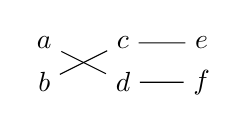
\begin{tikzpicture}
	nodes={draw, ultra thick}
	\node (a) at (0,0) {$a$};	\node (c) at (1,0) {$c$};	\node (e) at (2,0) {$e$};
	\node (b) at (0,-0.5) {$b$};	\node (d) at (1,-0.5) {$d$};	\node (f) at (2,-0.5) {$f$};
	\draw (a) -- (d) -- (f);
	\draw (b) -- (c) -- (e);
\end{tikzpicture}
\end{center}
\end{example}

From a game theoretic point of view, a matching is a subset $M$ of the strategy profiles where for each $i \in N$ and $a_i \in A_i$ there is exactly one $s \in M$ such that $s_i = a_i$, and hence $|M| = m$. 

For each $i, j \in N$, a matching $M$ induces a bijection $M_{ij} \in \bij(A_i, A_j)$ where, given $a_i \in A_i$, $M_{ij}(a_i)$ is the unique $a_j \in A_j$ such that there exists $s \in M$ with $s_i = a_i$ and $s_j = a_j$. For example given the matching in Example \ref{matchingeg}, $M_{31} = \bigl(\begin{smallmatrix} e & f \\ b & a \end{smallmatrix}\bigr)$.

\begin{lemma}
	$\{M_{ij}: i, j \in N\}$ is a groupoid. 
	\begin{proof}
		It follows by definition that for each $i, j, k \in N$, $M_{ii} = \id_{A_i}$, $M_{ij}^{-1} = M_{ji}$ and $M_{jk} \circ M_{ij} = M_{ik}$. Now for each $i, j, k, l \in N$, $M_{ij} \circ M_{ii} = M_{ij} = M_{jj} \circ M_{ij}$, $M_{kl} \circ (M_{jk} \circ M_{ij}) = M_{kl} \circ M_{ik} = M_{il} = M_{jl} \circ M_{ij} = (M_{kl} \circ M_{jk}) \circ M_{ij}$, $M_{ij} \circ M_{ij}^{-1} = M_{ij} \circ M_{ji} = M_{jj}$ and $M_{ij}^{-1} \circ M_{ij} = M_{ji} \circ M_{ij} = M_{ii}$.
	\end{proof}
\end{lemma}

Furthermore, for each $\pi \in S_N$, a matching $M$ induces a game bijection $\bigl(\pi; (M_{i\pi(i)})_{i \in N}\bigr) \in S_{\Gamma}$, which we denote as $M_{\pi}$. For example given the matching in Example \ref{matchingeg}, $M_{(13)} = \bigl((13) ; \bigl(\begin{smallmatrix} a & b \\ f & e \end{smallmatrix}\bigr), \bigl(\begin{smallmatrix} c & d \\ c & d \end{smallmatrix}\bigr), \bigl(\begin{smallmatrix} e & f \\ b & a \end{smallmatrix}\bigr)\bigr)$. 

For each $H \subseteq S_N$ and matching $M$ we denote the set $\{M_{\pi}: \pi \in H\}$ of bijections induced by $H$ as $M_H$. For example given a subgroup $G$ of $S_{\Gamma}$ we have $M_{\overrightarrow{G}} = \{M_{\pi}: \pi \in \overrightarrow{G}\}$. 

\begin{lemma} \label{matchinghomoprop}
	$M:S_N\rightarrow{S_{\Gamma}}$ is a homomorphism.
	\begin{proof}
		Let $\pi, \phi \in S_N$, then $M_{\phi} \circ M_{\pi} = \bigl(\phi; (M_{i\phi(i)})_{i \in N}\bigr) \circ \bigl(\pi; (M_{i\pi(i)})_{i \in N}\bigr) = \bigl(\phi \circ \pi; (M_{\pi(i)(\phi\circ\pi)(i)} \circ M_{i\pi(i)})_{i \in N}\bigr) \newline = \bigl(\phi \circ \pi; (M_{i(\phi\circ\pi)(i)})_{i \in N}\bigr) = M_{(\phi \circ \pi)}$.
	\end{proof}
\end{lemma}

\begin{corollary}
	$M_{\pi^{-1}} = M_{\pi}^{-1}$ for all $\pi \in S_N$.
\end{corollary}

\begin{lemma} \label{matchingfixedpointlemma}
	For each $\pi \in S_N$, $M_{\pi}(s) = s$ for all $s \in M$.
	\begin{proof}
		For each $i \in N$, $\bigl(M_{\pi}(s)\bigr)_i = M_{\pi^{-1}(i)i}(s_{\pi^{-1}(i)}) = s_i$.
	\end{proof}
\end{lemma}

If we relabel the strategies played in each $s \in M$ to be the same, giving players the same strategy labels, then each permutation $\pi \in S_N$ acts on our relabelled strategy profiles equivalently to how $M_{\pi}$ acts on our original strategy profiles. Hence a subgroup $G$ of $S_{\Gamma}$ acts on strategy profiles equivalently to permutations for some relabelling of the strategies precisely when $G = M_{\overrightarrow{G}}$ for some matching $M$, which we now establish occurs precisely when $G$ is strategy trivial. 

\begin{theorem} \label{strattrivmatchingthm}
	Let $G \leq S_{\Gamma}$ be player transitive. There exists a matching $M$ such that $M_{\overrightarrow{G}} = G$ if and only if $G$ is strategy trivial.
	\begin{proof}
		Suppose there exists a matching $M$ such that $M_{\overrightarrow{G}} = G$. That $M_{\overrightarrow{G}} \leq S_{\Gamma}$ follows from Lemma \ref{matchinghomoprop}. Now for each $i \in N$ and $g \in G_i$, $M_{ig(i)} = M_{ii} = \id_{A_i}$.
		
		Conversely suppose $G$ is strategy trivial. By Corollary \ref{NoahCor}, for each $i \in N$ and $\tau \in \overrightarrow{G}$ there exists $g_{i\tau(i)} \in \bij(A_i, A_{\tau(i)})$ such that $G = \{\bigl(\pi; (g_{i\pi(i)})_{i \in N}\bigr): \pi \in \overrightarrow{G}\}$. 
		
		Let $i \in N$ and $M = \{(g_{ij}(a_i))_{j \in N}: a_i \in A_i\}$. $M$ is a matching since for each $j \in N$ and $a_j \in A_j$, there exists a unique strategy $a_i \in A_i$ for player $i$ such that $g_{ij}(a_i) = a_j$. Furthermore $M$ is independent of $i$ since for each $k \in N$, $\bigl(g_{ij}(a_i)\bigr)_{j \in N} = \bigl((g_{kj} \circ g_{ik})(a_i)\bigr)_{j \in N}$. Hence $M_{kl} = g_{kl}$ for all $k, l \in N$, giving us $M_{\pi} = \bigl(\pi; (M_{i\pi(i)})_{i \in N}\bigr) = \bigl(\pi; (g_{i\pi(i)})_{i \in N}\bigr) \in G$ for all $\pi \in \overrightarrow{G}$.
	\end{proof} 
\end{theorem}

Hence weakly anonymous games may be characterised as follows, similarly for anonymous and fully anonymous games.

\begin{corollary}
	The following conditions are equivalent:
	\begin{enumerate}
		\item There exists weakly anonymous $\Gamma'$ such that $\Gamma \cong \Gamma'$;
		\item There exists player $n$-transitive and strategy trivial $G \leq \Gamma$ such that for each $i \in N$ and $g \in G_i$, $u_i = u_i \circ g$; and
		\item There exists a matching $M$ such that for each $i \in N$ and $\pi \in S_{N-\{i\}}$, $u_i = u_i \circ M_{\pi}$.
	\end{enumerate}
\end{corollary}

We denote by $M(n, m)$ the set of matchings for an $n$-player $m$-strategy game. 

\begin{example}
	\begin{enumerate}
		\item If $m = n = 2$ then, letting $A_1 = \{a, b\}$ and $A_2 = \{c, d\}$, 
		\begin{align*}
			M(2, 2) = \bigl\{\{(a, c), (b, d)\}, \{(a, d), (b, c)\}\bigr\}.
		\end{align*}
		\item If $m = 3$ and $n = 2$ then, letting $A_1 = \{a, b, c\}$ and $A_2 = \{d, e, f\}$, \
		\begin{align*}
			M(2, 3) = \bigl\{&\{(a, d), (b, e), (c, f)\}, \{(a, d), (b, f), (c, e)\}, \{(a, e), (b, d), (c, f)\}, \\
						&\{(a, e), (b, f), (c, d)\}, \{(a, f), (b, d), (c, e)\}, \{(a, f), (b, e), (c, d)\}\bigr\}.
		\end{align*}
	\end{enumerate}
\end{example}

There are a number of ways to count the number of matchings in $M(n, m)$. Below we present one, though note an alternative is to establish that $M(n, m) \cong \bij(A_1, A_2) \times \ldots \times \bij(A_{n-1}, A_n)$. %\newpage

\begin{lemma} \label{matchinglemma1}
	For each $n \geq 2$: $M(n, 2)$ is a partition of $A$; and $|M(n, 2)| = 2^{n-1}$.
	\begin{proof}
		For each $s \in A$, the profile $s'$ where each player swaps their strategy choice is the unique profile in $A$ such that $\{s, s'\} \in M(n, 2)$. Consequently $|M(n, 2)| = \frac{|A|}{2} = 2^{n-1}$. 
	\end{proof}
\end{lemma}

\begin{lemma} \label{matchinglemma2}
	For each $n \geq 2$ and $m \geq 3$, $|M(n, m)| = m^{n-1}|M(n, m-1)|$.
	\begin{proof}
		Let $i \in N$. Each $a_i$ can be matched with each $a_{-i} \in A_{-i}$ and $ |A_{-i}| = m^{n-1}$. Furthermore, for each $(a_i, a_{-i})$ there are $|M(n, m-1)|$ ways to match the remaining $m-1$ strategies of the $n$ players.
	\end{proof}
\end{lemma}

\begin{theorem}
	For each $m, n \geq 2$, $|M(n, m)| = (m!)^{n-1}$.
	\begin{proof}
		This follows inductively from Lemmas \ref{matchinglemma1} and \ref{matchinglemma2}.
	\end{proof}
\end{theorem}
